\documentclass[letter,12pt]{article}
\usepackage[margin=2.3cm]{geometry}
\usepackage{parskip}
\usepackage{tikz}
\usepackage{amsmath}
\usepackage{amssymb}
\usepackage{algorithmic}
\usepackage{algorithm}
\usepackage{amsthm}


\begin{document}
Name: Yan, Zi \\
Course: CIS 502 \\
Assignment: HW2 \\
\line(1,0){400}
%Write your content here


\section*{Problem 1}
\paragraph*{a.)}
No.
In the figure \ref{p1a}, a minimum-bottleneck tree can be \{(c,d), (d,b),
(b,e), (a,b)\}, but the minimum spanning tree is \{(a,b), (a,c), (a,d),
(b,e)\}. 

\begin{figure}[!h]
\caption{example}
\label{p1a}
\center
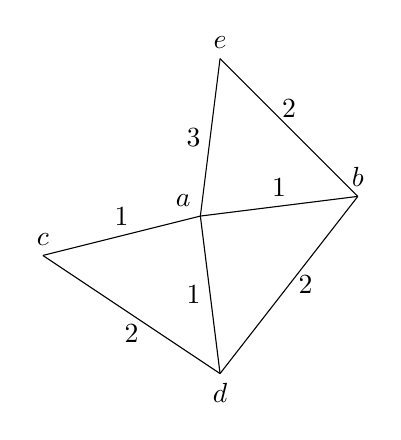
\begin{tikzpicture}
  \coordinate [label=170:$a$] (A) at (0,0);
  \coordinate [label=$b$] (B) at (2,0.25);
  \coordinate [label=$c$] (C) at (-2, -0.5);
  \coordinate [label=below:$d$] (D) at (0.25, -2);
  \coordinate [label=$e$] (E) at (0.25, 2);
  
  \draw (A) -- node[above] {1} (B);
  \draw (A) -- node[above] {1} (C);
  \draw (A) -- node[left] {1} (D);
  \draw (A) -- node[left] {3} (E);
  \draw (C) -- node[below] {2} (D);
  \draw (D) -- node[right] {2} (B);
  \draw (B) -- node[above] {2} (E);
\end{tikzpicture}
\end{figure}

\paragraph*{b.)}
Yes.
Suppose not. Let $T=(V, E')$ be the minimum spanning tree of the 
graph $G$, and $T'=(V, E'')$ be the minimum-bottleneck tree of $G$,
where $T$ and $T'$ are not identical. The difference is that $e \neq e'$
and $w_e < w_{e'}$, where $e \in E''$ is the most weighted edge in $T'$,
and $e' \in E'$ is the most weighted edge in $T$, but the rest edges of
two spanning tree are the same. From the assumption, we can show
that $\sum\limits_{e \in E'} w_e > \sum\limits_{e \in E''} w_e$. But this 
contradicts the fact that $T$ is MST.

\paragraph*{c.)} We can simply use Kruskal's Algorithm to find a 
minimum spanning tree in $O(m\log n)$ time. And the MST can be
regarded as a minimum-bottleneck tree.

\paragraph*{d.)} We can combine binary search and DFS to implement
the algorithm. Briefly, we use binary search to find a minimum 
bottleneck weight, using DFS to verify whether all the edges weighted 
no greater than this weight can make the original graph connected,
namely forming a spanning tree. 

\begin{proof}
Because DFS will provide a subgraph which makes all the nodes 
connected, if the original graph is connected. And once the binary
search can give a $w_{max}$ that makes the graph with all edge weights
less than or equal to $w_{max}$ connected, the DFS-MOD will also give
a connected subgraph which can be regarded as a spanning tree. As 
the binary search goes on, a minimum $w_{max}$ can be found that
it is the minimum weight and the graph with all edge weights no greater
than it will still be connected. At this time, DFS-MOD will provide
a minimum-bottleneck tree.

The binary search will take $O(\log m)$ time, but DFS-MOD will only
visit half of the graph at first and half of the unvisited graph or the
visited half in the subsequent steps. Therefore, the total runtime
will be $\sum\limits_{i=1}O(\frac{m+n}{2^i}) = O(m+n)=O(n+m\log n)$
\end{proof}

\begin{algorithm}
\caption{Using DFS to find minimum-bottleneck tree}
\begin{algorithmic}
\STATE \textbf{FIND\_MBT($G$)}
\WHILE{there are still more than one vertex in $G$}
\STATE Let $w_{max}$ = the median number of all existing edge 
weights
\STATE VERIFY-WEIGHT($G, w_{max}$)
\IF{$w_{max}$ is a valid weight}
    \STATE Remove all the unvisited edges from $G$
\ELSE 
    \STATE Regard all visited edges and vertices as a single node in the
following steps
\ENDIF
\ENDWHILE
\STATE The vertices and remaining edges consist of minimum 
bottleneck tree
\end{algorithmic}
\end{algorithm}

\begin{algorithm}
\begin{algorithmic}
\STATE VERIFY-WEIGHT($G, w_{max}$)
\FOR{each vertex $u \in V$}
    \STATE visited[$u$] = \FALSE
\ENDFOR
\STATE $v$ = any vertex picked from $V$
\STATE DFS-MOD($v$, $w_{max}$)
\FOR{each vertex $u \in V$}
    \IF{visited[$u$] == \FALSE}
        \RETURN "not a valid weight"
        \ELSE \RETURN "a valid weight"
    \ENDIF
\ENDFOR
\end{algorithmic}
\end{algorithm}

\begin{algorithm}
\begin{algorithmic}
\STATE DFS-MOD($u, w_{max}$)
\STATE visited[$u$] = \TRUE
\FOR{each $v \in$Adj[$u$]}
\IF{\NOT visited[$v$] \AND $w(u,v) \le w_{max}$}
\STATE DFS-MOD($v, w_{max}$)
\ENDIF
\ENDFOR
\end{algorithmic}
\end{algorithm}

\section*{Problem 2}
\paragraph*{(a)} It is true. Suppose not. Assume MACS (minimum 
altitude connected subgraph) has a distinct edge from MST (minimum 
spanning tree), connecting two nodes $i$ and $j$ to form a 
\textit{winter-optimal} path. This means that a edge $e_{\text{MACS}}$
in MACS, which is the highest edge in the path from $i$ to $j$, is 
lower than the highest edge $e_{\text{MST}}$ in MST. Therefore,
$\sum\limits_{e \in E_{\text{MACS}}}a_e < \sum\limits_{e \in 
 E_{\text{MST}}}a_e$, which contradicts the fact of MST.

%
%
%MST (minimum 
%spanning tree) has a distinct edge $e_{\text{MST}}$ from MACS 
%(minimum altitude connected subgraph), connecting two disjoint sets of 
%vertices $S$ and $V-S$, and the rest edges are the same. There are two 
%cases here.
%\begin{itemize}
%    \item[1.] $A(e_{\text{MST}}) > A(e_{\text{MACS}})$. Therefore, 
%    $\sum\limits_{e \in E_{\text{MACS}}}a_e < \sum\limits_{e \in 
%    E_{\text{MST}}}a_e$, but this contradicts that MST has the minimum 
%    total edge weight.
%    \item[2.] $A(e_{\text{MST}}) < A(e_{\text{MACS}})$. Therefore, 
%    between town $i$ and $j$, where $i \in S$ and $j \in (V-S)$ and $i$ 
%    and $j$ are directly connected by $e_{\text{MST}}$, in the MACS, the 
%    path between them will have at least $e_{\text{MACS}}$ maximum 
%    weight. In such a condition, the MACS is not optimal, which 
%    contradicts the assumption.
%\end{itemize}
%So, the MST, with respect to the edge weights $a_e$, is a MACS.

\paragraph*{(b)}
It is true. Suppose not. Assume the MACS contains no edge from the 
MST. This means in a cycle the highest edge $e_h$, which connects
the vertices $i$ and $j$, is in the MACS. Therefore removing $e_h$ and 
connecting $i$ and $j$ with the ``longer way" will form a better 
\textit{winter-optimal} path than before. This contradicts the 
assumption.


\section*{Problem 3}
Initially we need an additional array $r$, and $r$ is identical to array 
$d$, where $r_i = d_i$, and it means that $v_i$ can still form $r_i$
edges to other vertices.

The algorithm is that from $v_1$ to $v_n$ you pick a vertex one by one.
Every time a vertex $v_i$ is chosen, you choose any $r_i$ other vertices,
each of which has its subscript $j$ larger than $i$ with non-zero $r_j$ 
value, to form $r_i$ edges for each, then decrease the corresponding
$r_j$ by 1. After you go through all the vertices, all the element in array 
$r$ should be zero, otherwise the graph $G$ will contain either multiple 
edges between the same pair of nodes or self-loop edges, or both.

The algorithm maintains that if $G$ will not contain either multiple 
edges between the same pair of nodes or self-loop edges, at vertex 
$v_i$, each vertex $v_j$, where $j<i$, have connected to $d_j$ vertices 
with $r_j = 0$, and $r_i \le (n-i)$.
\begin{proof}
\textbf{Base:} When picking $v_1$, it is trivial.

\textbf{Induction Step:} Assume at vertex $v_i$, every vertex $v_j$,
where $j<i$, have connected to $d_j$ vertices with $r_j = 0$, and 
$r_i \le (n-i)$. So at vertex $v_{i+1}$, according to the operation
in $i$th step, there should be no less than $r_i$ vertices with non-zero
$r$, otherwise $v_i$ will have not enough vertices to connect to,
which leads to either self-loop edges or multiple edges between $v_i$
and any other vertices, therefore contradicts the assumption. Then, 
$v_i$ can form $r_i$ edges from itself to any $r_i$ vertices, decreasing
$r_i$ to zero. For $r_{i+1}$, it should be no greater than $n-i$,
otherwise, multiple edges between $v_{i+1}$ and any other vertices
or self-loop edges will be formed, which contradicts the assumption.
Consequently, at $v_{i+1}$, the property still maintains.

At $v_n$, all the other vertices have their $r$ equal to zero, and $r_i \le 
(n-n) = 0$. It means every vertex $v_i$ connects to $d_i$ different
vertices with no multiple edge between the same pair of vertices and
no self-loop edge.
\end{proof}

%Suppose not, then there will be multiple edges between the same pair of 
%nodes, or self-loop edges. First, we discuss multiple edge between the 
%same pair of nodes, which means between $v_i$ and $v_j$, where $i < 
%j$, there are at least two edges. But from the algorithm above, we only 
%form exact one edge to $v_j$ when we are at $v_i$, therefore, the other
%edges are formed when we are at $v_j$. But this contradicts with our
%algorithm. Second, we discuss self-loop edges. But from the algorithm, 
%before we reach the last vertex, no self-loop edge is formed, therefore, 
%the self-loop edges will be formed when we finish the last vertex, which
%means there will be one vertex with non-zero degree. This contradicts
%the assumption.

For each vertex $v_i$, $O(d_i)$ is used to form edges and decrease 
$r_i$, so the total runtime of the algorithm should be 
$\sum\limits_{k=1}^n O(d_k) + O(n)= O(n+m)$.

\section*{Problem 4}
The algorithm maintains a property that every time a vertex $v$ is 
visited, dist[$v$] will hold the current shortest distance from $s$ to
$v$, and num[$v$] indicates the number of shortest paths from $s$
to $v$ with distance dist[$v$].

%Suppose not. Assume at $i$th step, the path from $s$ to $u$ is not
%the shortest one, but there is one edge $(k', j)$ instead of $(k, j)$ will
%make the path from $s$ to $k'$ to $u$ shorter than the one from $s$
%to $k$ to $u$. Therefore, dist[$k'$] + $w_{k',j} <$ dist[$k$] + $w_{k,j}$.
%And this contradicts with lines 14-20 in the algorithm.
%
%Meanwhile, lines 17-19 ensure when there are alternately shortest paths,
%num[$v$] will take those paths into account. 

\begin{proof}
\textbf{Base:} At the beginning, only $s$ is visited, therefore, dist[$s$]
=0, num[$s$]=1, and the dists of all the other nodes are $\infty$ and
the nums of them are 0.

\textbf{Induction Step:} At $i$th step, all the visited nodes will hold 
shortest distance from $s$ and how many of them. Then, at $(i+1)$th 
step, a vertex $v$ will be visited from a vertex $u$, which is visited at 
$i$ step, on the following two conditions:

\begin{itemize}
    \item $v$ is not visited. At this time, at least one shortest path from
    $s$ to $v$ is established. But the actual number of shortest paths is
    just the number of shortest paths from $s$ to $u$.
    \item $v$ is visited before. So if another shortest path from $s$ via
    $u$ to $v$ exists, the total number of shortest paths should be 
    accumulated. And Line 15 finishes the job.
\end{itemize}

Finally, at vertex $t$, the shortest distance from $s$ and the number of
the of paths will maintain.
\end{proof}

Because the algorithm just add some constant time operations, Line 
12-16, the runtime should be still $O(n+m)$.

\begin{algorithm}
\begin{algorithmic}[1]
\STATE \textbf{BFS-SHORTEST}($s$)
\STATE Set visited[$s$] = \TRUE \;and visited[$v$] = \FALSE \;for all
other $v$
\STATE Set dist[$s$] = 0 and dist[$v$] =$\infty$ for all other $v$
\STATE Set num[$s$] = 1 and num[$v$] = 0 for all other $v$
\STATE Add $s$ to Queue $Q$
\WHILE{$Q$ is not empty}
\STATE Let $u$ = Dequeue($Q$)
\FOR{all $v$ which is adjacent to $u$}
\IF{visited[$v$] == \FALSE}
\STATE Enqueue($Q$, $v$)
\STATE visited[$v$] = \TRUE
\STATE dist[$v$] = dist[$u$] + 1
\STATE num[$v$] = num[$u$];
\ELSE
\IF{dist[$v$] == dist[$u$] + 1}
\STATE num[$v$] = num[$v$] + num[$u$]
\ENDIF
\ENDIF
\ENDFOR
\ENDWHILE
\RETURN num[$t$]
\end{algorithmic}
\end{algorithm}
\end{document}